\chapter{Mockups}
\label{a:prototipos}

\section{Interfaces do utilizador}
\label{interfaces}

\subsection{Autenticação}

Quando se acede à página oficial da aplicação, é possível ver a descrição do produto, funcionalidades, planos entre outros. É também a partir da página do produto que o utilizador consegue realizar a autenticação na plataforma.

Representado nas Figuras \ref{10q-login} e \ref{10q-registo} temos as interfaces que dizem respeito à autenticação do utilizador.

Quando se efectua o \textit{login} na plataforma, o utilizador é apresentado com a interface representada na Figura \ref{10q-login}, onde é necessário introduzir o email e password associados à sua conta. Caso as credenciais não estejam corretas, o utilizador é notificado para esse efeito.



\begin{figure}[ht!]
	\begin{center}
		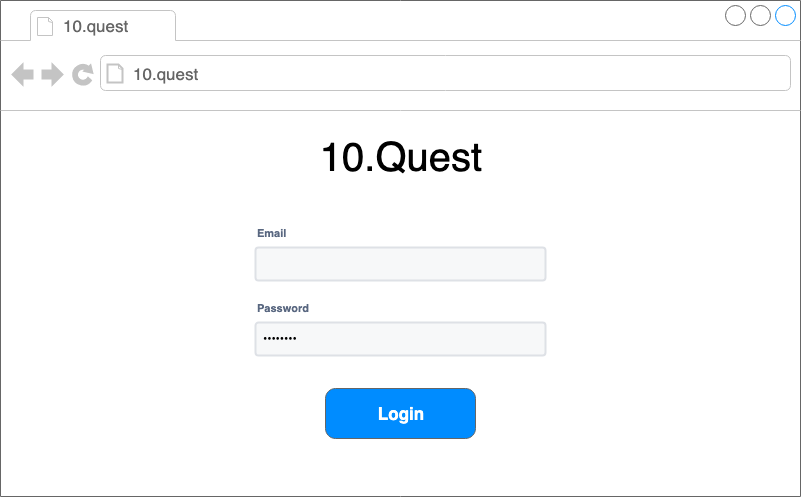
\includegraphics[width=1\textwidth]{img/prototipos/1.png}
		\caption{10.quest - Login}
		\label{10q-login}
	\end{center}
\end{figure}


Para criar uma conta nova, é necessário aceder à pagina de registo da plataforma. Como podemos ver na Figura \ref{10q-registo}  para criar uma conta nove é necessário introduzir o nome, nome da empresa, email, nome de utilizador e password.

\begin{figure}[ht!]
	\begin{center}
		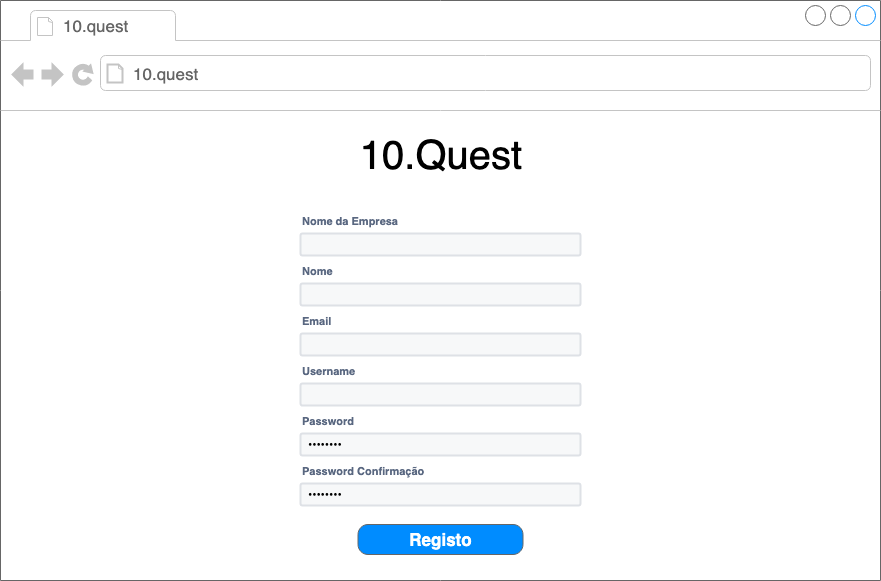
\includegraphics[width=1\textwidth]{img/prototipos/2.png}
		\caption{10.quest - Registo}
		\label{10q-registo}
	\end{center}
\end{figure}

\newpage

\subsection{Página Inicial}

Representado na Figura \ref{10q-home} temos a página principal da plataforma. A partir da página inicial um utilizador autenticado tem acesso a todas as funcionalidades principais do sistema representadas na Figura \ref{d:altonivel}, na secção \ref{rf}.

A partir da páginas principal o utilizador têm acesso às formações, questionários e concursos mais recentes (i. e. os ultimos que criou ou editou) e respectivo estado e, no fundo da página, é ainda possível observar algumas estatísticas globais relativas aos mesmos que serão definidas no segundo semestre.

\begin{figure}[ht!]
	\begin{center}
		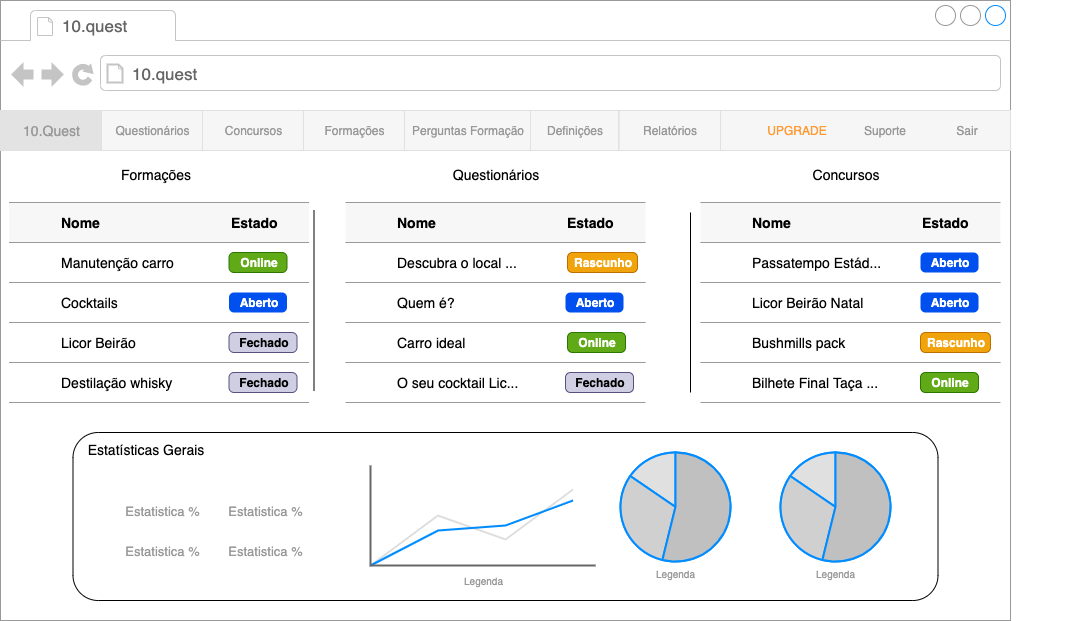
\includegraphics[width=1\textwidth]{img/prototipos/home.png}
		\caption{10.quest - Página Inicial}
		\label{10q-home}
	\end{center}
\end{figure}
\newpage

\subsection{Questionários}

Na Figura  \ref{10q-listaQ} temos página principal dos questionários. Nesta página estão listados todos os questionários associados à conta do utilizador. Para cada questionário é possível ver a data de inicio, data de fim, o estado actual do questionário e ainda alguns dados estatísticos que irão ser definidos no segundo semestre.
Para  apagar um ou mais questionários o utilizador tem que marcar cada um deles e depois carregar no botão para eliminar os questionários. É ainda possível pesquisar um questionário por nome.

\begin{figure}[ht!]
	\begin{center}
		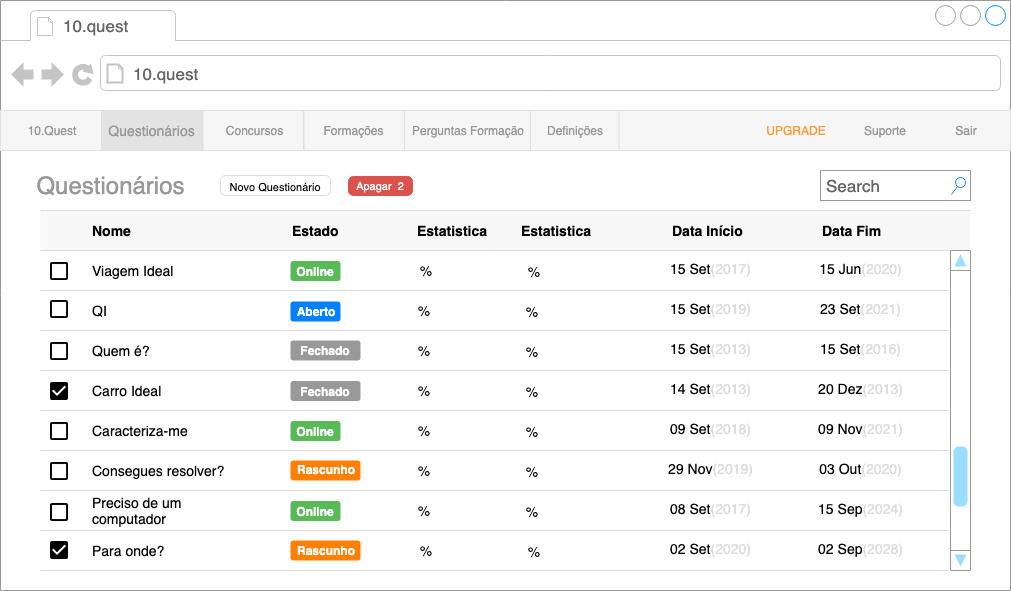
\includegraphics[width=1\textwidth]{img/prototipos/4.png}
		\caption{10.quest - Lista de Questionários }
		\label{10q-listaQ}
	\end{center}
\end{figure}


Para criar um novo questionário, o utilizador carrega no botão para criar um novo questionário e é redirecionado para a página de criação de um questionário, representado na Figura \ref{10q-questoes}.

Numa primeira instência o utilizador tem de criar um conjunto de questões que serão utilizadas para criar o querstionário. Na Figura \ref{10q-Nquestao} podemos observar a criação de uma nova questão.

\clearpage


\mbox{}
\begin{figure}[ht!]
	\begin{center}
		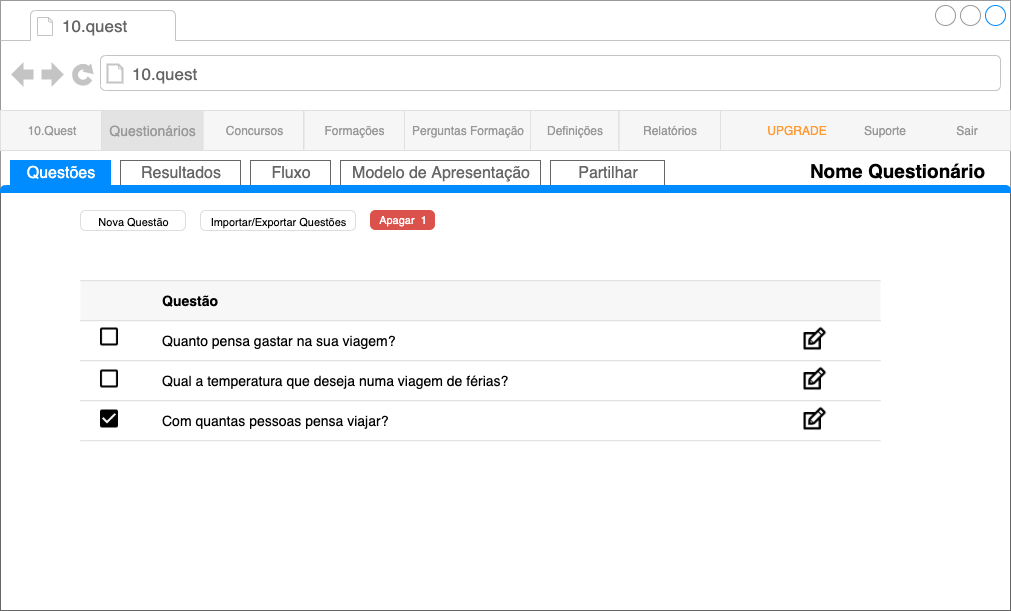
\includegraphics[width=1\textwidth]{img/prototipos/13.png}
		\caption{10.quest - Criar Questionário (Lista de questões)}
		\label{10q-questoes}
	\end{center}
\end{figure}

\begin{figure}[ht!]
	\begin{center}
		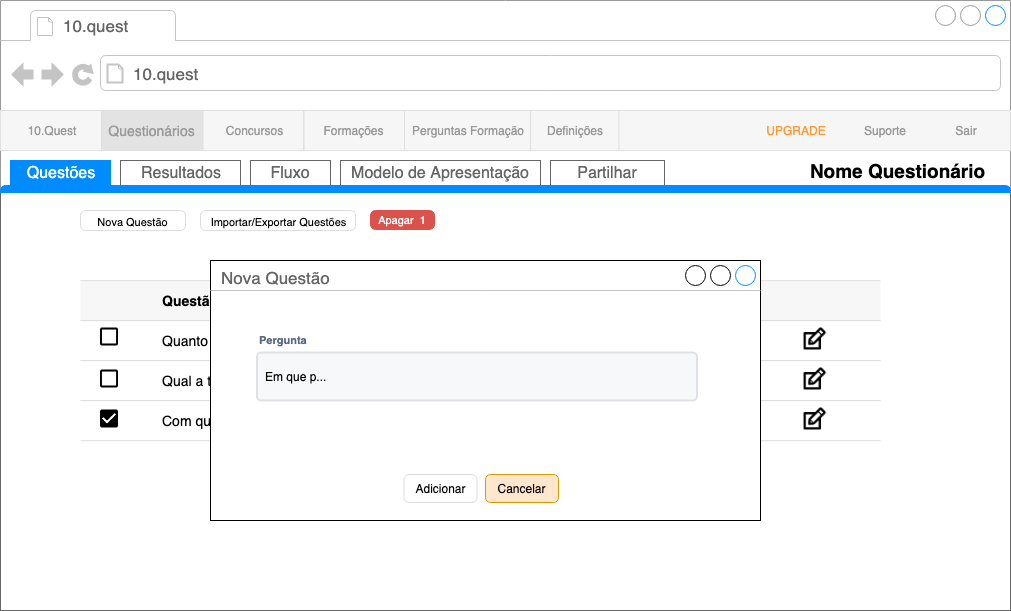
\includegraphics[width=1\textwidth]{img/prototipos/14.png}
		\caption{10.quest - Criar Questionário (Nova Questão) }
		\label{10q-Nquestao}
	\end{center}
\end{figure}
\newpage

Representado na Figura \ref{10q-result} temos a lista de resultados possíveis do questionário. Depois de terminada a criação de todas as questões pretendidas para a criação do questionário, o utilizador segue para a criação dos resultados possíveis para o questionário. 
Representado na Figura \ref{10q-Nresult} temos a criação de um novo resultado. Para criar um novo resutaldo o utilizador necessita de introduzir obrigatóriamente um título e uma tag. O utilizador pode também, opcionalmente, associar um link e/ou um ficheiro de imagem, audio ou vídeo.

\begin{figure}[ht!]
	\begin{center}
		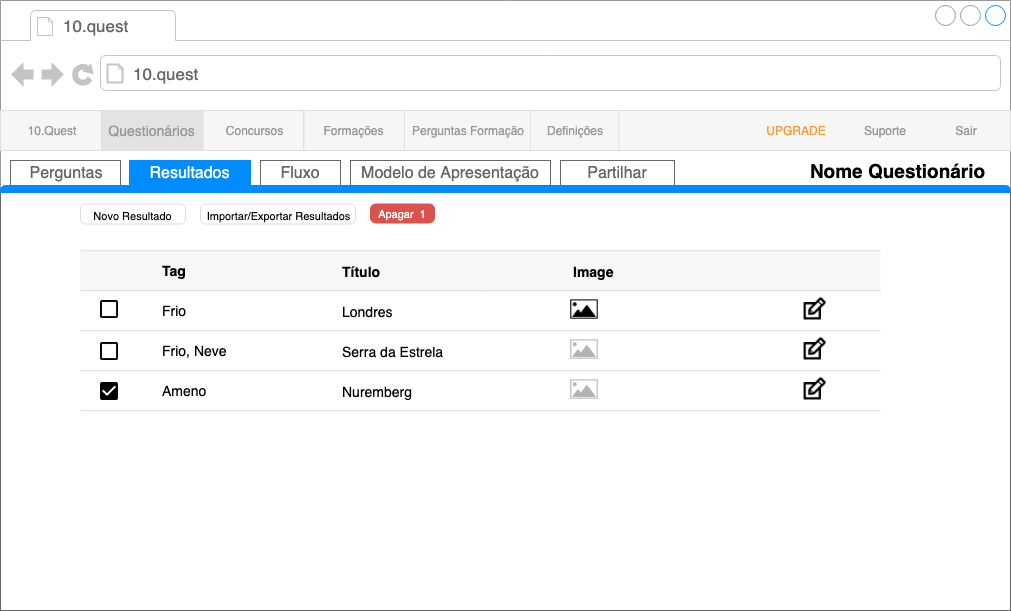
\includegraphics[width=1\textwidth]{img/prototipos/15.png}
		\caption{10.quest - Criar Questionário (Lista de Resultados)}
		\label{10q-result}
	\end{center}
\end{figure}

\begin{figure}[ht!]
	\begin{center}
		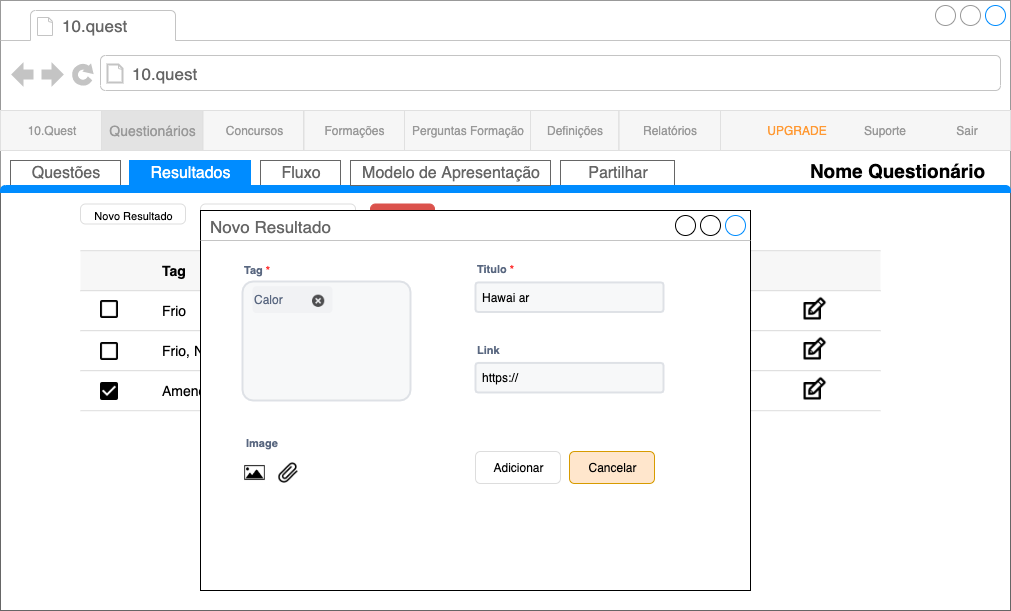
\includegraphics[width=1\textwidth]{img/prototipos/16.png}
		\caption{10.quest - Criar Questionário (Novo Resultado)}
		\label{10q-Nresult}
	\end{center}
\end{figure}
\newpage

\begin{figure}[ht!]
	\begin{center}
		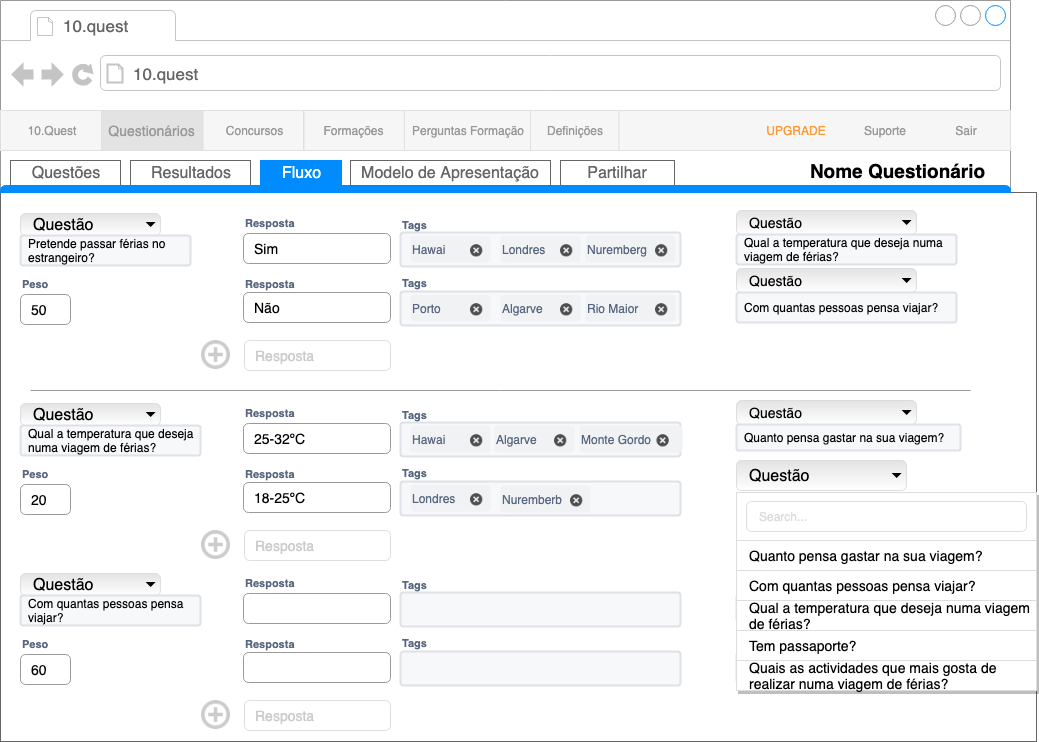
\includegraphics[width=1\textwidth]{img/prototipos/17.png}
		\caption{10.quest - Criar Questionário (Fluxo de questões)}
		\label{10q-}
	\end{center}
\end{figure}

\newpage

\subsection{Concursos}

\begin{figure}[ht!]
	\begin{center}
		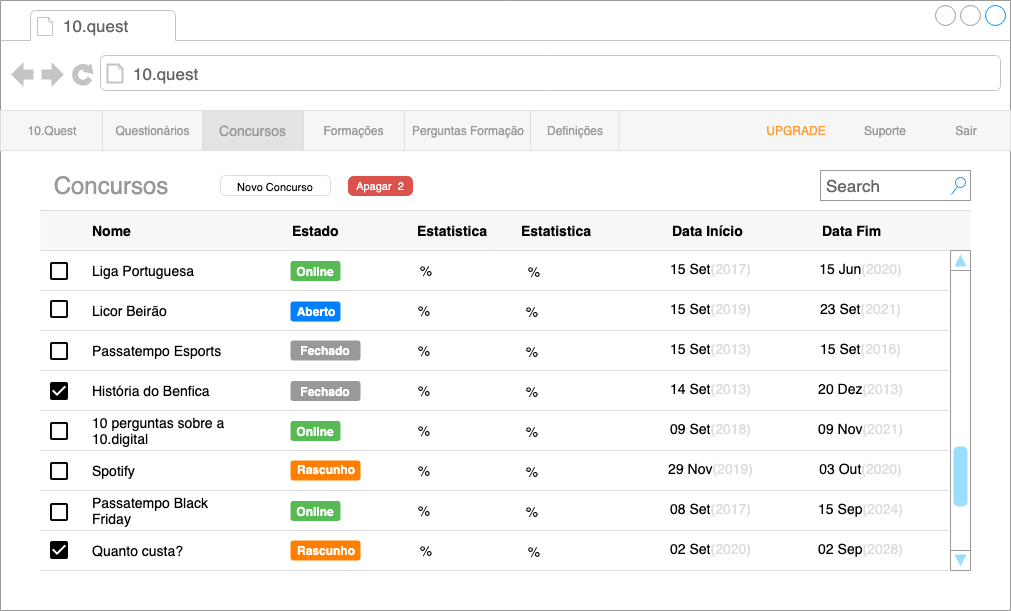
\includegraphics[width=1\textwidth]{img/prototipos/5.png}
		\caption{10.quest - Lista de Concursos}
		\label{10q-}
	\end{center}
\end{figure}

\begin{figure}[ht!]
	\begin{center}
		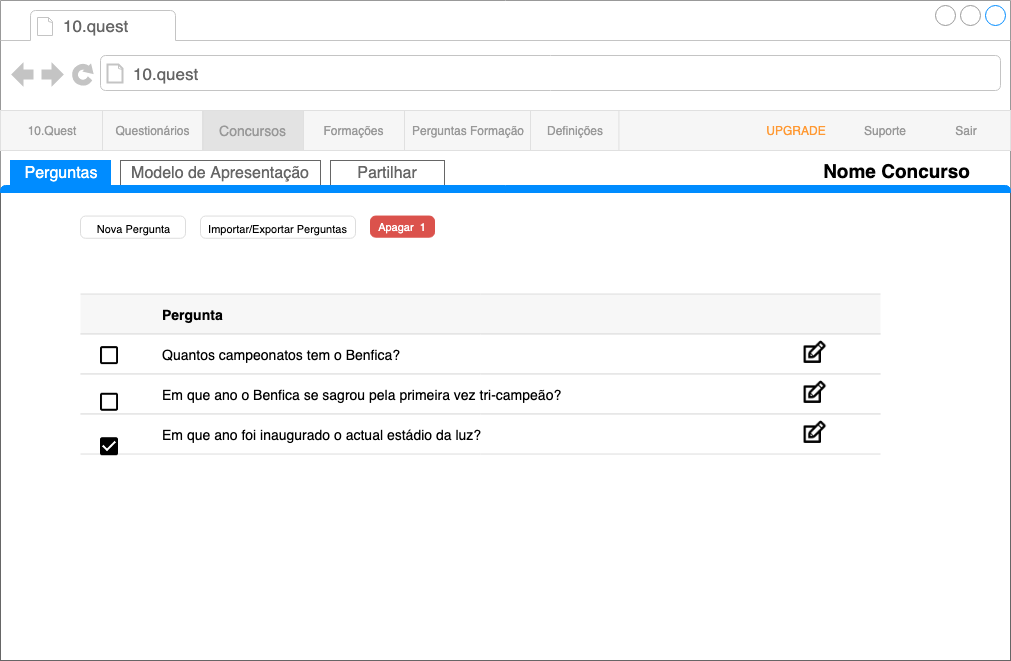
\includegraphics[width=1\textwidth]{img/prototipos/18.png}
		\caption{10.quest - Criar Concurso(Lista de Perguntas)}
		\label{10q-}
	\end{center}
\end{figure}


\begin{figure}[ht!]
	\begin{center}
		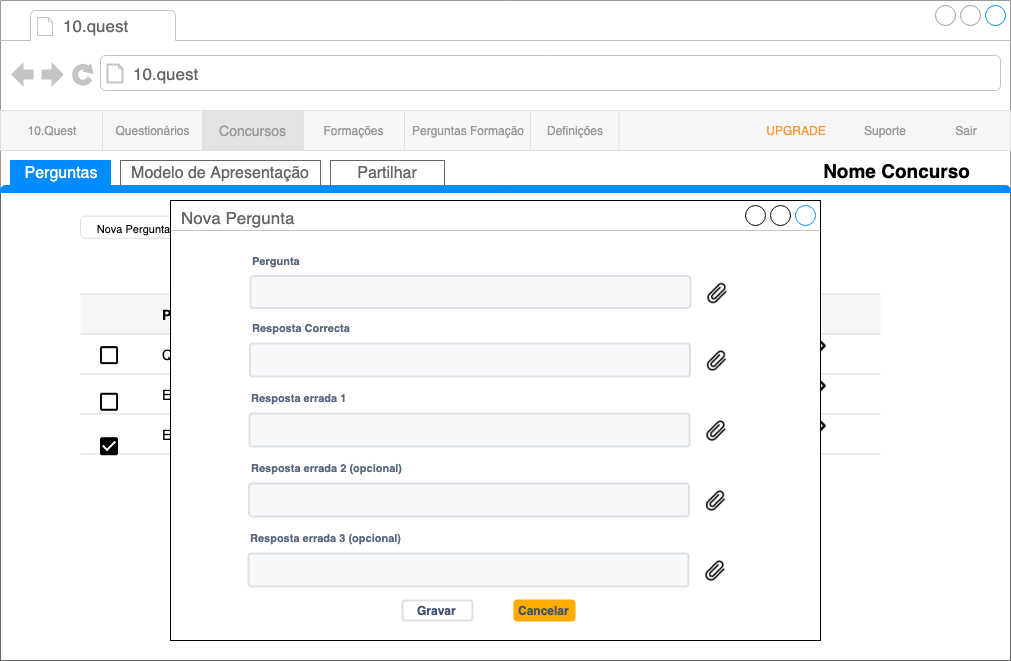
\includegraphics[width=1\textwidth]{img/prototipos/19.png}
		\caption{10.quest - Criar Concurso(Nova Pergunta)}
		\label{10q-}
	\end{center}
\end{figure}

\newpage

\subsection{Formações}

\begin{figure}[ht!]
	\begin{center}
		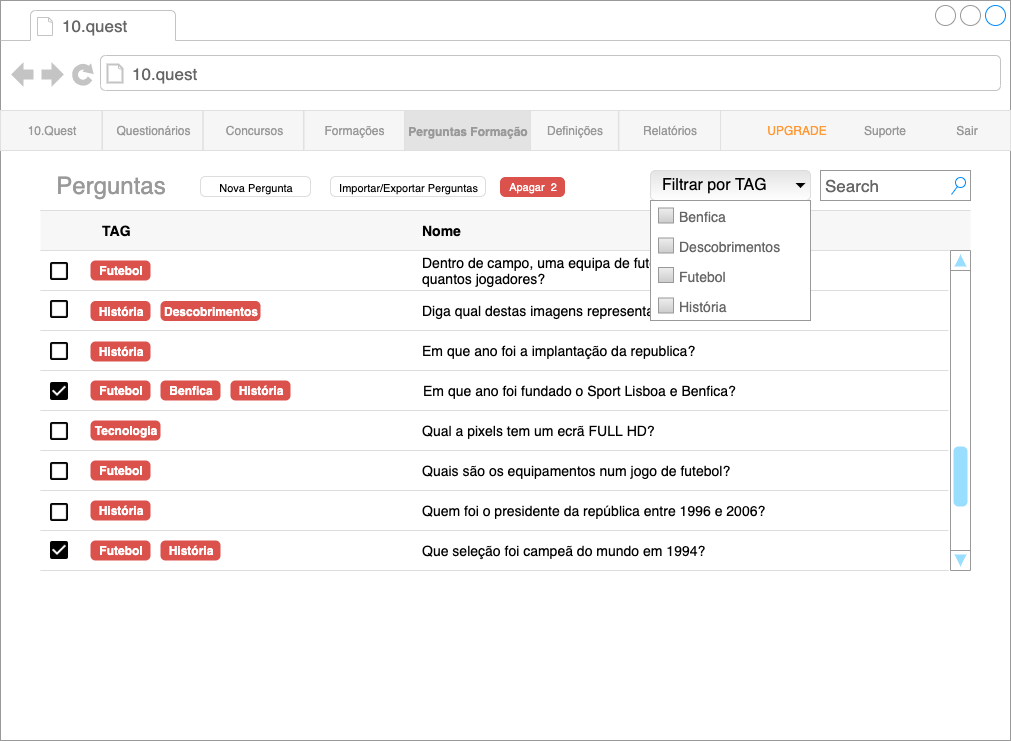
\includegraphics[width=1\textwidth]{img/prototipos/6.png}
		\caption{10.quest - Lista de Perguntas para formação}
		\label{10q-}
	\end{center}
\end{figure}

\begin{figure}[ht!]
	\begin{center}
		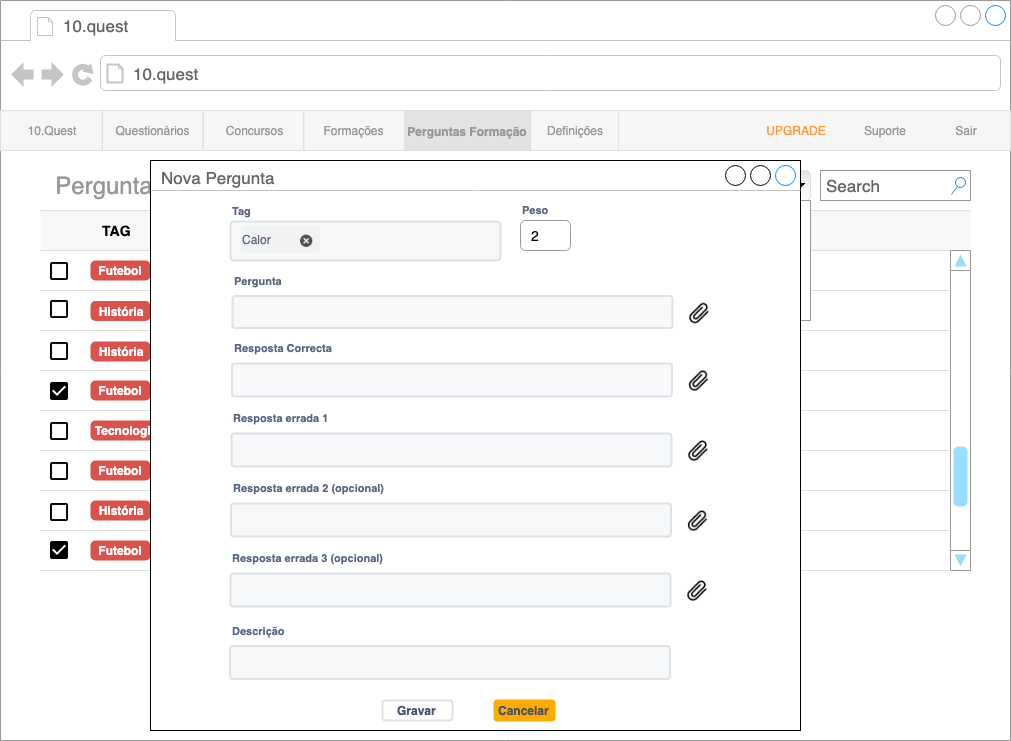
\includegraphics[width=1\textwidth]{img/prototipos/7.png}
		\caption{10.quest - Nova Pergunta para formação}
		\label{10q-}
	\end{center}
\end{figure}

\begin{figure}[ht!]
	\begin{center}
		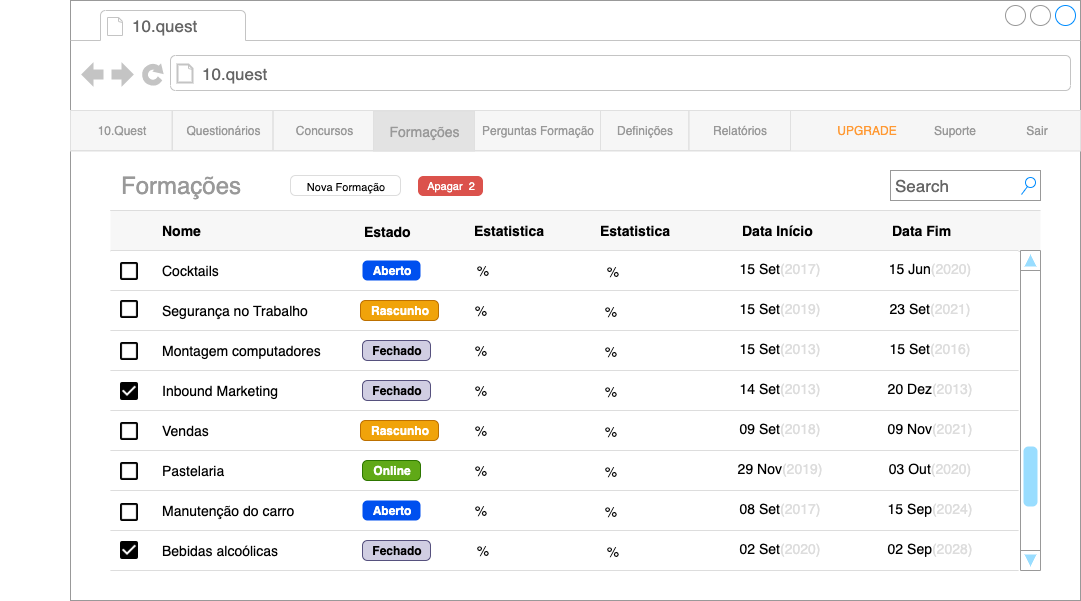
\includegraphics[width=1\textwidth]{img/prototipos/8.png}
		\caption{10.quest - Lista de Formações}
		\label{10q-}
	\end{center}
\end{figure}

\begin{figure}[ht!]
	\begin{center}
		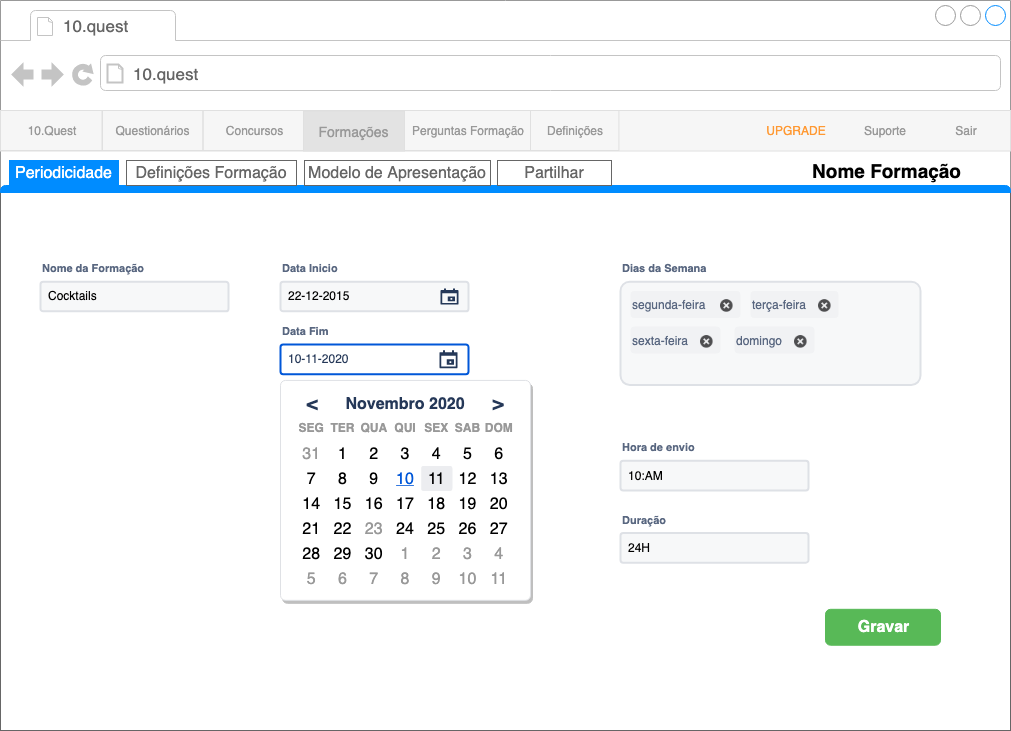
\includegraphics[width=1\textwidth]{img/prototipos/9.png}
		\caption{10.quest - Criar Formação (Periodicidade)}
		\label{10q-}
	\end{center}
\end{figure}

\begin{figure}[ht!]
	\begin{center}
		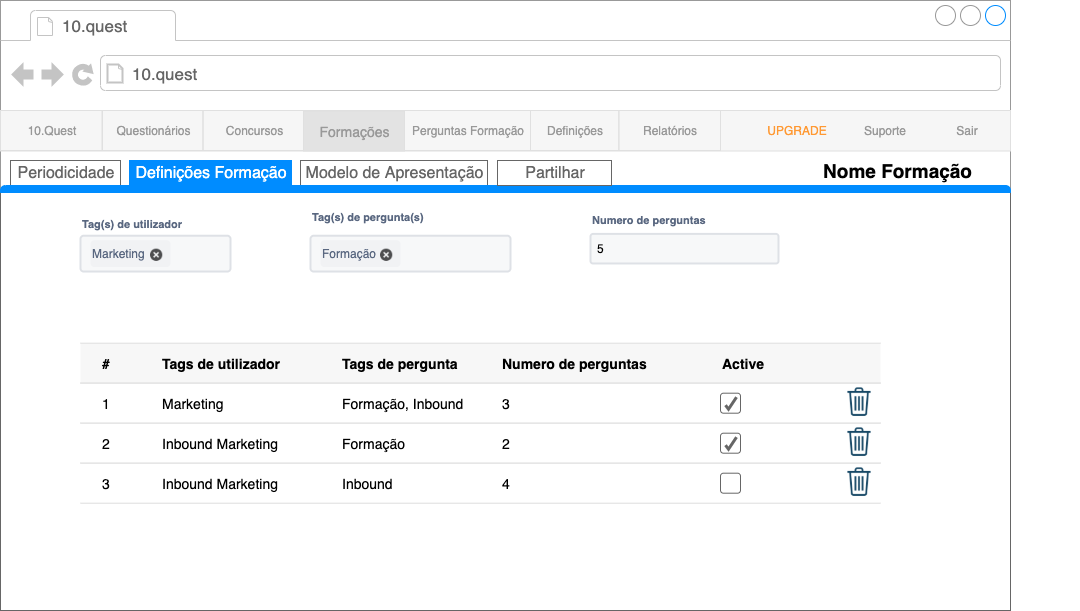
\includegraphics[width=1\textwidth]{img/prototipos/10.png}
		\caption{10.quest - Criar Formação (Definições da Formação)}
		\label{10q-}
	\end{center}
\end{figure}

\begin{figure}[ht!]
	\begin{center}
		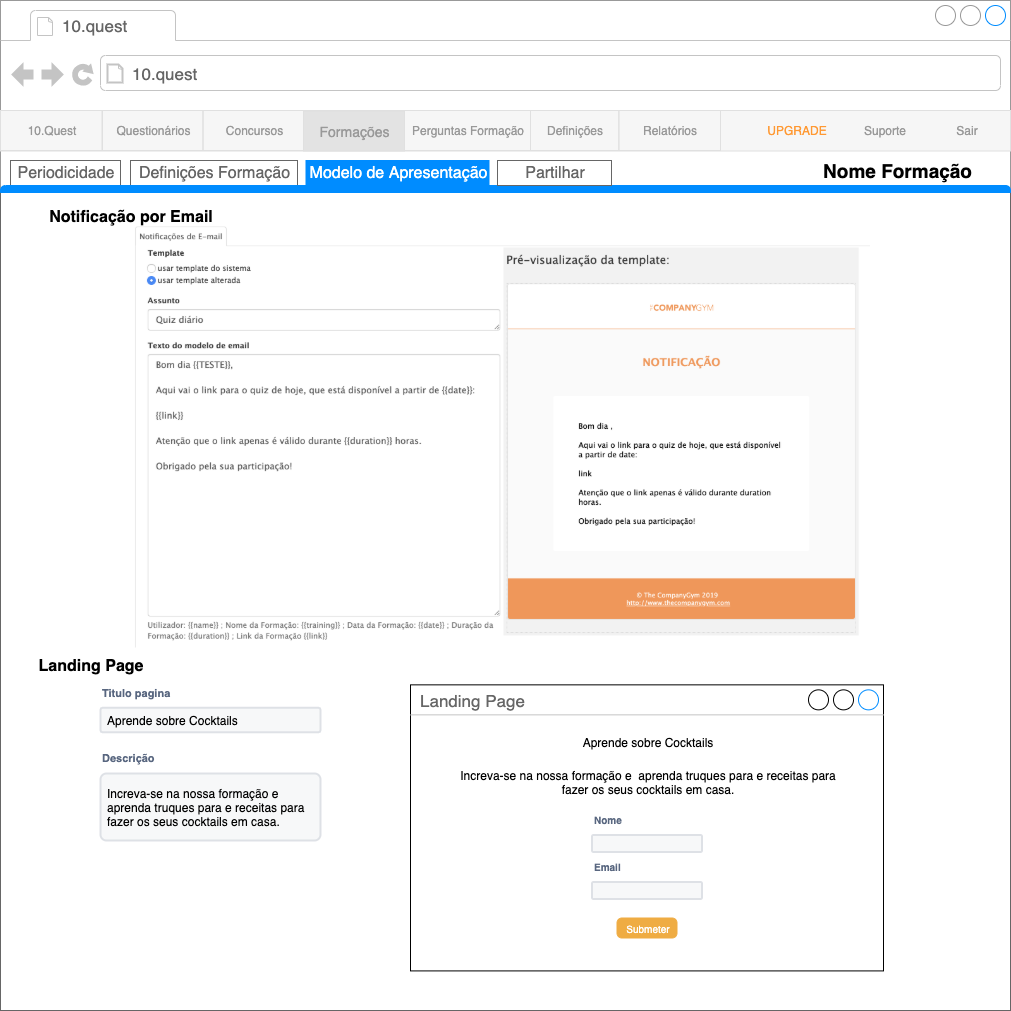
\includegraphics[width=1\textwidth]{img/prototipos/11.png}
		\caption{10.quest - Criar Formação (Modelo de Apresentação)}
		\label{10q-}
	\end{center}
\end{figure}

\begin{figure}[ht!]
	\begin{center}
		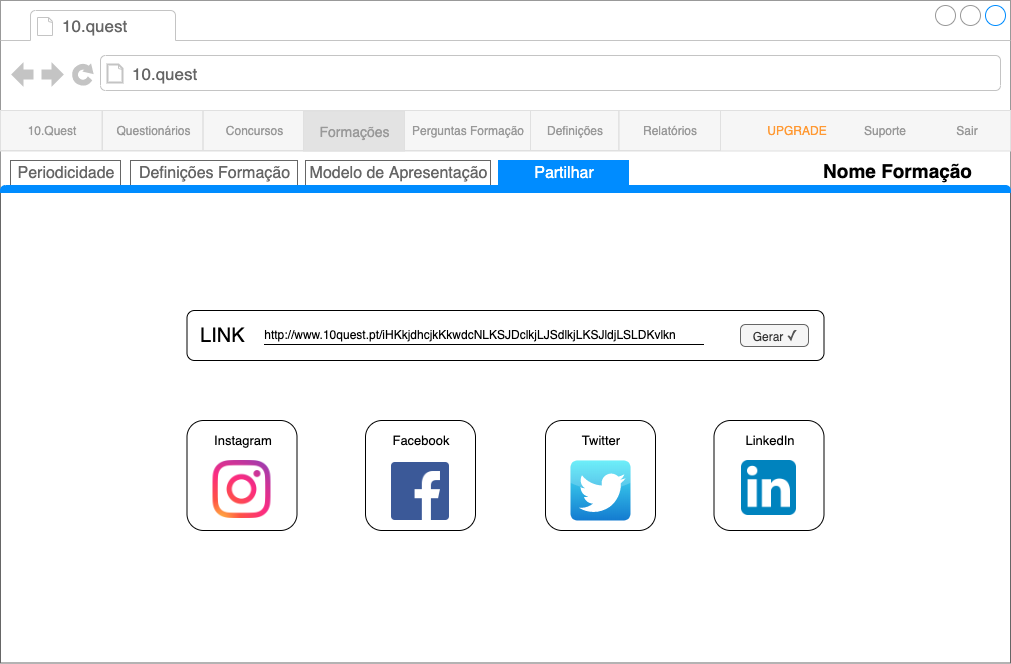
\includegraphics[width=1\textwidth]{img/prototipos/12.png}
		\caption{10.quest - Partilhar Formação}
		\label{10q-}
	\end{center}
\end{figure}


\newpage

\subsection{Definições e Plano de funcionalidades}


\begin{figure}[ht!]
	\begin{center}
		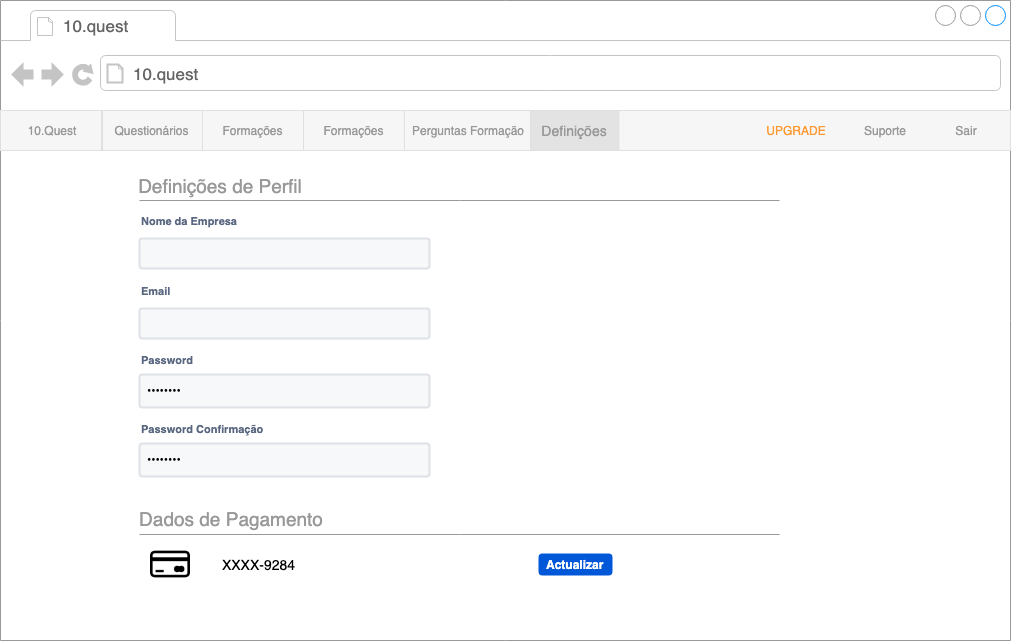
\includegraphics[width=1\textwidth]{img/prototipos/20.png}
		\caption{10.quest - Definições}
		\label{10q-}
	\end{center}
\end{figure}

\begin{figure}[ht!]
	\begin{center}
		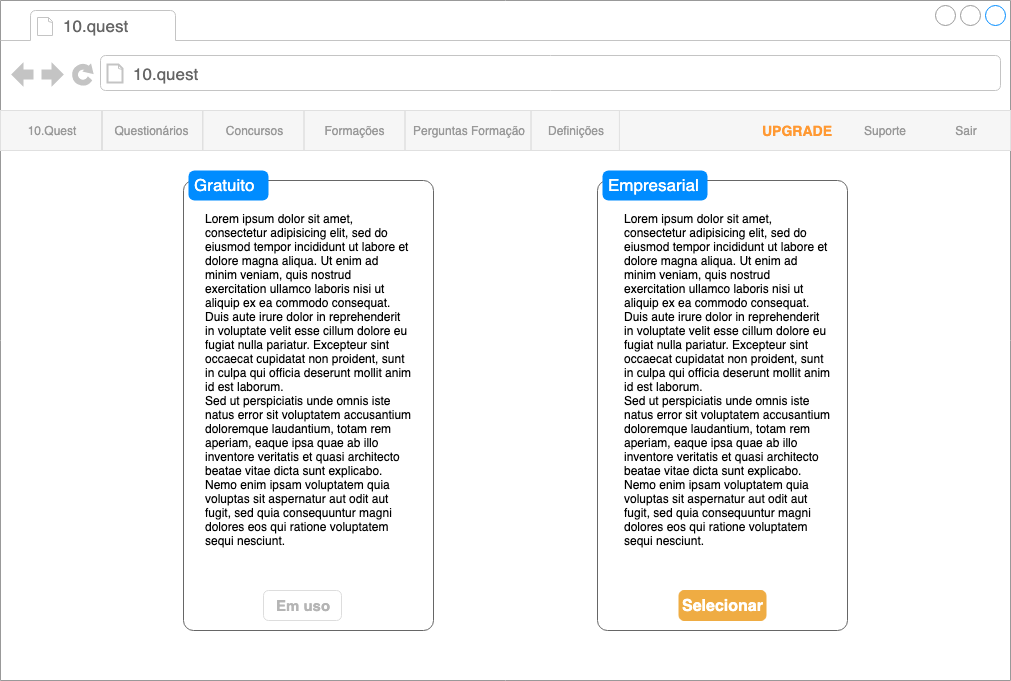
\includegraphics[width=1\textwidth]{img/prototipos/21.png}
		\caption{10.quest - Planos e Preços}
		\label{10q-}
	\end{center}
\end{figure}




